\title{System Dynamics:  Exercise 3 - Adaptation in Chemotaxis}
\author{Ryan Spangler}
\date{\today}

\documentclass[12pt]{article}

\usepackage{graphicx}

\begin{document}
\maketitle

\section{Approach}

For this exercise I chose to make a simple model of biological adaptation.  Adaptation is a word that is used in many ways throughout many fields, but in this particular case I am referring to it in the way that \cite{Alon} defines it, that a particular quality of a system returns to a set point after a perturbation, compensating for the perturbation with respect to whatever quality is being fixed.  In the case of this exercise I am choosing the subject to be the biological circuit involved in bacterial chemotaxis.   (Most of the following information is gleaned from \cite{Alon} and \cite{Fall}, as well as other supplementary descriptions).  

There are many facets of bacterial chemotaxis, and it is different for different species and so forth, but there is a basic description of a general mechanism that more or less forms the backbone of the process of sensing and responding to chemical gradients.  The cell lives in an environment of chemicals, and navigates through this world by traveling towards things it can consume and away from things that are poisonous or harmful.  Subtle differences in the gradient of a particular chemical or chorus of chemicals can be enough to point a simple bacteria to nutritional salvation, and bacteria are amazingly good at finding food in a sea of conflicting chemical signals.  When the means of transport is isolated, it turns out that this cell has only two distinct modes of motion, mediated by the rotation of a host of long, thin flagella.  When the flagella rotate counterclockwise, the cell is propelled forward in a straight line.  When the flagella rotate clockwise however, the cell tumbles around, not going anywhere, but ending up oriented in a new, random direction.  The inevitable counterclockwise rotation following this pulse of clockwise tumbling sends the cell speeding off in a new direction.  So that's it, two modes: straight, or tumbling.  The tumbling is effectively random, so there is no preference to a certain direction as a result of one tumble or another.  Every orientation is equally probable.  So to a certain degree the fact that the cell can get anywhere specific appears to be somewhat of a mystery, with such limited means of locomotion, much less with such success as the cell enjoys.  The secret lies in a system that links the contour of a chemical gradient with the frequency at which it initiates tumbling.  

There are three main proteins involved in this circuit:  cheW, cheB, and cheY, with a supporting role from cheB and cheZ (most of the proteins involved in chemotaxis share the prefix 'che').  The cycle goes like this: there is a receptor column that spans the membrane, activating cheW in the presence of various repellents or deactivating in the presence of attractants.  Activated cheW phosphorylates cheB and cheY.  Phosphorylation is common as a kind of tagging for proteins, often either activating or deactivating them or inducing conformational shifts that are detected by still other proteins.  In this case, the additional phosphate activates both cheB and cheY.  CheY triggers the flagellar motor to increase the frequency of spinning clockwise, inducing tumbling.  CheB on the other hand removes methyl groups from cheW, only if the cheW is active.  The more methyl groups that are attached to a particular cheW the more likely it is to become active, so by removing them, phosphorylated cheB deactivates cheW.  This is the source of the main balancing feedback loop of the system:  active cheW activates cheB (through phosphorylation), which deactivates cheW (through demethylation).  There are other factors which methylate cheW at a constant rate (cheR) and dephosphorylate cheB and cheY at a constant rate (cheZ).  In this way, in the absence of activated cheW, there will be a lack of phosphorylated cheB, which will leave the phosphorylation of cheW by cheR unchecked, growing until some threshhold is reached where cheW is activating again, adding phosphates to the cheB's, which remove all the excess methyl groups from the cheW's and return the activation back to normal.  

One point should be made about cell dynamics: all of the elements involved in this circuit or any circuit exist at some kind of concentration, meaning at any one time there is a population of active cheW and a population of inactive cheW; there are phosphorylated cheY's and cheB's floating around and there are unphosphorylated ones.  At all times methyl groups are being added to cheW and methyl groups are being removed, and it is the balance between all of these simultaneous events that we describe as the process of living.  At all times there is a multitude of parallel balances between different proteins and states of those proteins at work in the cell.  

\section{Reference Behavior Pattern}

In all of this, the behavior I was looking to model (RBP) was that the activation of cheW (which led to the increase in tumbling through phosphorylating cheY) would spike with the sudden addition of repellent, and then if no change in the gradient was made from that point on, the cheW activation would return to its original level (through the demethylation of cheW by cheB that had been phosphorylated by active cheW).  This is known as exact adaptation, where any perturbation is eventually absorbed in the pursuit of maintaining a specific level of a given quantity.  No matter what the stimulus, if kept constant the response would always return back to the same level.  In this way the activation history of cheW is more an indication of a {\em change} in stimulus rather than any particular {\em level} of stimulus.  

This is the basic behavior I was looking for when designing the model, and this is what guided me to model the chemical gradient as a step function, where at a certain time step a repellent would be added, whereupon the cheW activation would increase, triggering a series of events which returned the cheW activation back to its normal level, in spite of the fact that the repellent remained at a higher state than it was before.

The graph I used as the RBP is Figure 7.8 on page 144 of \cite{Alon}, which basically describes graphically exactly this.

\section{Process}

I went through a series of failed models before arriving at some moderate form of success, and with each iteration I removed what I had come to conclude as unnecessary complication.  My first model had nine stocks, my second five, and my final model has only three, a drastic simplification from the original attempt.  My initial model contained a pair of stocks for each kind of thing, one for the activated/phosphorylated/methylated version and one for the deactivated/dephosphorylated/demethylated one.  There was one flow that connected the inactive stock to the active stock for each pair, which was positive when there was a net activation happening and negative for a net deactivation.  This was problematic in that there was no simple way to prevent any of the stocks from going negative, even though what I was trying to model by having one flow between two stocks was a fixed amount of a substance vascillating between one of two states.  Ideally, if there is no more of a quantity left in a particular stock there is none of it to flow into the other stock, so nothing can change until some flows back into it from the other stock.  In order to do this as a Vensim model it would be necessary to implement a conditional IF THEN ELSE for each stock and flow, in order to check for the zero condition and fail to flow or change if the value is zero.  This is doable, but was an indication to me that I was on the wrong path.  I would rather the model worked endogenously, than working because of the interplay of a spattering of IF THEN ELSE statements.  

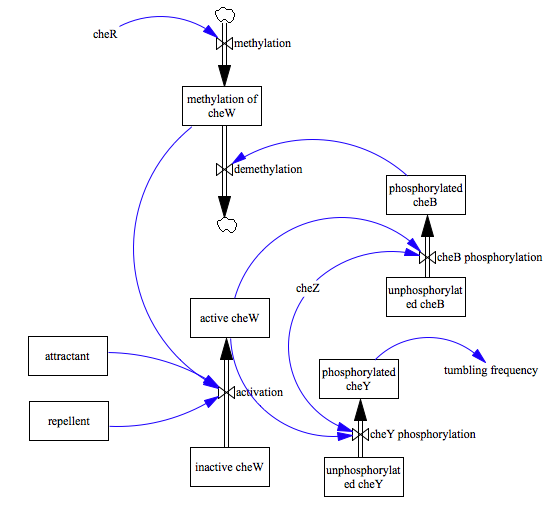
\includegraphics[scale=0.7]{dualstock.png}

The second model approached each active counterpart as a stock, and ignored the inactive versions.  Nothing in the model depended on the quantity of the inactive counterparts anyway, another indication that the dual-stock approach was misguided.  This one was better, but suffered from a chronic tendency to oscillate chaotically out of control.  Once again, a fresh approach was needed.  The main insight I made was to use autoregulation, where the inflow to an active state depended inversely on the amount residing in the stock, and the outflow depended directly on that same amount.  This led to a stable pattern of activity for all the various variables, seeking out a particular level to balance the number flowing in and out of the stock in this way.  No matter what the starting conditions, if left to their own devices all of the stocks would seek out some ideal level.  This idea of autoregulation formed a stable basis for all of the interdependencies between these stocks that would be added later.  

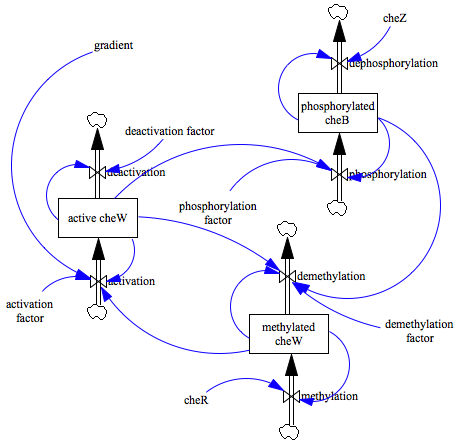
\includegraphics[scale=0.71]{autoregulation.png}

As you can see, the three stocks are active cheW, phosphorylated cheB and methylated cheW.  Active cheW contributes to the phosphorylation of cheB, and cheB collaborates with the activity of cheW to demethylate cheW.  The more cheW is methylated the more likely it is to be activated.  This is the core loop of the model, in addition to supplementary autoregulatory loops between each stock and its respective inflows and outflows.   Its balancing force is the heart of the adaptation mechanism.

The main parameters are the factors for the inflows and outflows of the three stocks, and the gradient, which is modeled as a step function.  The gradient is zero until time 42, when it kicks on to 25.0 and remains that way for the duration of the experiment.  This models the sudden addition of repellent to the solution the cell occupies.  

\section{Verification and Validation}

Verification was an elaborate process for all of the models, which in the instance of the failed ones you could say I verified that the models did {\em not} reflect the RBP.  Each period of verification I spent trying all kinds of things to make it work (adding or removing arrows, tweaking parameters endlessly, etc) before I could definitively declare that I had to start over, that the anomalies I was seeing were because of flaws in the model and not the conspiring of model parameters, or some other nonessential source.  Each time I started over was a blessing however, because I used the failures of the previous ones to guide my design into something more appropriate to the system I was modeling. Each time my model became simpler and more direct, and I was grateful for the insights I had gained by the earlier failures.   

One of the best approaches to verification I found was to guess what the effect of changing a particular parameter value to be.  I would say to myself, ``What will happen if I increase this parameter by 0.1?'' and see if I was right.  The most consterning ones were the ones that seemed to have no effect at all on the behavior, until I passed a certain threshhold and everything would fall apart.  I learned which parameters were the most sensitive and which ones had the least impact.  

At some point I tired of the routine of modifying a parameter in Vensim, running the model, selecting the graph, clicking on the items to graph, etc over and over and over every time I wanted to see how something changed, so I wrote my own program to do batch runs over a varying parameter.  I first wrote a simple stock and flow composition library based on the the process used in the hand integration lab from the beginning of the course.  Then I built programmatically the model as I had specified it in Vensim.  Here is an excerpt of how the model is defined with the simple stock and flow library (the code is in Ruby):

\begin{verbatim}
@model = Model.new

@active_cheW = @model.add_stock('active cheW', 10.0)
@methylated_cheW = @model.add_stock('methylated cheW', 10.0)
@phosphorylated_cheB = @model.add_stock('phosphorylated cheB', 10.0)
@exogenous = Stock.new('exogenous', 0.0)

@activation = @model.add_flow('activation', @exogenous, @active_cheW)
@deactivation = @model.add_flow('deactivation', @active_cheW, @exogenous)
@methylation = @model.add_flow('methylation', @exogenous, @methylated_cheW)
    ....

@gradient = @model.add_parameter('gradient', 0.0)
@activation_factor = @model.add_parameter('activation factor', 20.0)
@deactivation_factor = @model.add_parameter('deactivation factor', 0.1)
    ....

@activation.define { (@methylated_cheW.level - @gradient.level) 
    * @activation_factor.level / @active_cheW.level}
@deactivation.define { @deactivation_factor.level * @active_cheW.level }
@methylation.define { @cheR.level / @methylated_cheW.level }
    ....
\end{verbatim}

First the model is created, then the various stocks, flows and parameters are added to it with ``add\_flow'', ``add\_stock'' and ``add\_parameter''.  Then the ``define'' method is used to specify what the relationships are between the elements.  Once the model is defined in this way, it can be called with ``run(timesteps)'' to run the model for the given number of time steps and output the three stocks to a graph.  Once I had this going, I did a validation on the new program by running each it and Vensim for identical time steps with identical parameters and comparing the graphs until they were identical.  Then I tested it with other parameters and sure enough, I had modeled Vensim!  A decidedly easier task than modeling adaptation in chemotaxis it turns out.  Once I had that going I added the ability to track a given parameter in even steps across a defined range.  So I was able to ask it to generate all the graphs from a demethylation factor of 0.000005 to 0.00005 in 5 steps, for example.  This would result in 5 graphs in a row, and I could apprehend immediately what the effect of a given parameter was.  

Here is the series of graphs generated from the above specification (with active cheW as red, methylated cheW as green and phosphorylated cheB as blue):

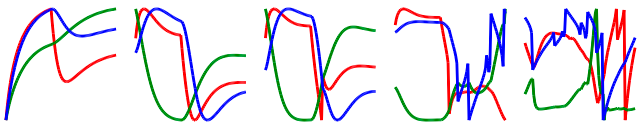
\includegraphics[scale=0.55]{seriesthree.png}

This shows the demethylation factor crossing over into chaotic behavior.  Of all the parameters, the demethylation factor was the most sensitive.

Rendering a series turned out to be a great aide to understanding the effect of a particular parameter value on the behavior of the model, but what I really wanted was to see how parameter values interact.  I imagine an n-dimensional space where each axis is bounded by the range in which it exhibits rational behavior, and the totality of all of the combinations of all the possible parameter values and their relationships forming a landscape describing the entirety of the models behavior.  What I had created by rendering a series of parameter values was a one dimensional projection of this total model space against the chosen parameter for a given range.  By adding another parameter this would become a plane through this space, and I would be able to see a two dimensional matrix of graphs, one parameter varying per axis.  This turned out to be a straightforward extension of the system I was already using:

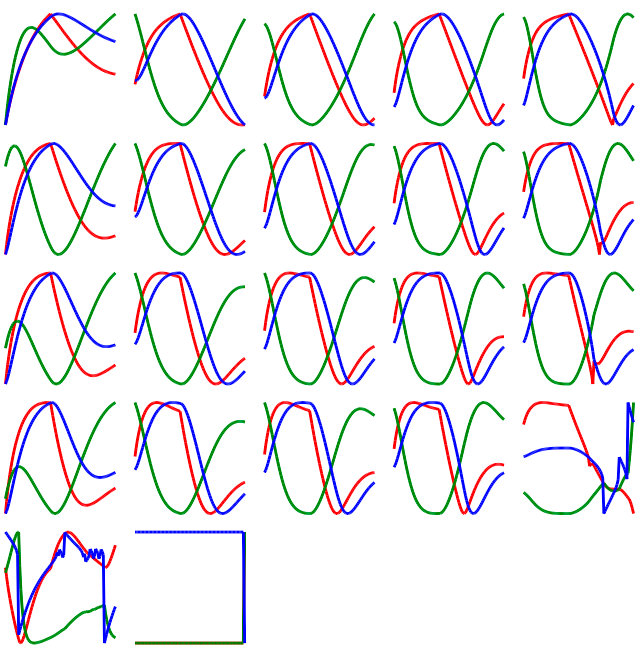
\includegraphics[scale=0.55]{matrix.png}

As is evident in this figure, the graph matrix proved to be useful in finding the boundaries of a system as well.

\section{Results}

I was able to achieve some degree of adaptation, but not exact adaptation.  Meaning that after the introduction of the repellent, the cheW activation would spike immediately, inducing the phosphorylization of cheB to rise, leading to a swifter removal of the methylation of cheW which raised the threshhold at which cheW became active again, restoring the cheW activation to some measure of its previous lower level, before the introduction of the repellent.  No matter how I tweaked the model I could not achieve exact adaptation, where the activation of cheW return back to exactly its former level.  

Here is an example of the model's ideal behavior (this is a case where the signal is an attractant, rather than a repellent.  The behavior is inverse and symmetrical, meaning the cheW activation goes down initially instead of up.):

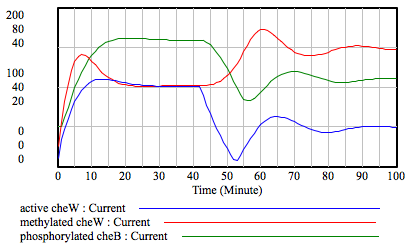
\includegraphics[scale=0.8]{ideal.png}

In this graph the model returns to about half of its original level after the crash.  After the initial drop the level rises swiftly, then evens out with graceful oscillations.  

As previously mentioned, the demethylation factor proved to be the most sensitive.  It demanded to be at a very low rate, and worked well only for a narrow band of about an order of magnitude.  Also, it was the parameter that led most quickly into chaotic chopping motions like so:

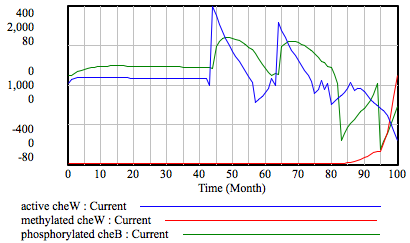
\includegraphics[scale=0.8]{chaotic.png}

The chaos I determined was mostly due to when the parameters happened to lead one of the equations to a negative value.  I pondered what ways I could use to ensure that the values were never negative, or better, cast the problem in a way that negative values could make sense, and therefore not go to unnatural strains to avoid it.  I also wondered whether the ability to become negative pointed to a basic flaw in my entire scheme, but it worked well enough in the range that it was well behaved that I tolerated the existence of these undefined and nonsensical zones.  I am not yet experienced enough yet to know whether all models have these zones of pain where nothing makes sense, or if you're model really is supposed to work under all conditions.  This is still an open question to me.  

\section{Transfer and Learning}

I learned many things above and beyond the basic background for this exercise, many things I did not expect to learn.  One of the big realizations was the value of autoregulation.  \cite{Alon} discusses autoregulation as one of the most basic and most important network motifs that is used everywhere throughout the living cell.  The chemical basis of autoregulation is well documented, but it was revealed to me clearly the necessity of it in its contribution to the dynamics.  Autoregulation provides a stable basis to respond to triggers or signals from the outside environment.  

Another thing I learned is how much more time is spent on model verification and validation than in actually building a model.  In the series of attempts I created the model quickly, and it took a great deal more time actually determining if the model worked, much less how well it related to actual data.  Validating a model especially I can see taking years in extreme cases, especially since so many things go into it.  Correlating it to actual data is just one part.  First you have to find the data, which is probably incomplete or from several unrelated and incongruous studies which need to be arranged and normalized.  I can see the design of a model demanding certain data be gathered that don't exist yet, and leading to experiments targeted at procuring particular kinds of data for use with a model.  Then you have to reckon with all the flaws that are revealed by actually comparing your model's behavior to real data.  Quite a strenuous process, and I feel that even though I did a great deal of work, I really only got far enough to {\em glimpse} how much work there is left to do.  

One of the elaborations on this model I would like to try is to have the gradient signal vary beyond a simple on/off.  I used this signal as a basis to demonstrate the existence or non-existence of adaptation, but really a cell in the world is surrounded by a constantly shifting gradient of a host of chemicals it is paying attention to.  It would be interesting to have a continuous signal for a gradient, to simulate approaching or distancing itself from a particular chemical source.

All in all a fruitful endeavor, and I would like to continue my work on the simple modeling system.  I am most interested in developing new ways to interact with and visualize the behavior of the model.  I feel like making a matrix of resultant graphs is really only scratching the surface in representing what is really a continuous and rich multi-dimensional space that the model occupies.  And I see models as having a great benefit not just in scientific endeavor as a means to make predictions, but also as a means to approach and understand what would otherwise be cryptic pursuits.  The more a model can be direct and immediately comprehensible to people the greater its impact in terms of the general population.  Beyond being a technical challenge it is also a deeply creative challenge, and I hope, a helpful one.

\section{Equations}

\begin{verbatim}
active cheW = 10.0
methylated cheW = 10.0
phosphorylated cheB = 10.0

gradient = 0.0
activation factor = 20.0
deactivation factor = 0.1
demethylation factor = 0.00002
phosphorylation factor = 1.0
cheR = 20.1
cheZ = 0.05

activation = (methylated cheW - gradient) * activation factor 
   / active cheW
deactivation = deactivation factor * active cheW 
methylation = cheR / methylated cheW 
demethylation = phosphorylated cheB * demethylation factor 
    * methylated cheW * active cheW 
cheB phosphorylation = active cheW * phosphorylation factor 
    / phosphorylated cheB 
cheB dephosphorylation = cheZ * phosphorylated cheB 
gradient = time step > 42 ? 25.0 : 0.0 
\end{verbatim}

\bibliographystyle{plain}
\bibliography{chemotaxis}

\end{document}
